\section{Day 4}
\subsection{Lecture 1}

\noindent \textit{Disclaimer: today had a lot of spectral sequences, and I'm not sure how coherent the writing is below here. I tried to get the spectral sequences correct, but I may have missed some important language helping us make these.}

Yesterday we computed a homotopy fixed point spectral sequence. Suppose that $C_2\acts\calE$ where $\calE$ is a spectrum. 

$$E_2^{s,t} = H^s(C_2;\pi_t \calE)\Rightarrow \pi_{t-s}\calE^{hC_2}.$$

\DeclareSseqGroup\etatowertwo{}{
    \class[rectangle](0,0)
    \foreach\i in {1,...,11}{
        \class[fill = white](\i,\i)
        \structline(\i-1,\i-1,-1)(\i,\i,-1)
    }
}
\begin{sseqdata}[name = HFPSSd2,x range ={0}{16},y range = {0}{4},xscale = .5,Adams grading]
    \foreach \k in {-2,...,4}{
        \etatowertwo({4*\k},0)
    }
    \d[wongorange]3 (-4,0)
    \replacesource[rectangle]
    \d[wongorange]3(4,0)
    \replacesource[rectangle]
    \d[wongorange]3(12,0)
    \replacesource[rectangle]
    \foreach \n in {1,...,6}{
        \d[wongorange]3 ({-4+\n},\n)
        \d[wongorange]3({4+\n},\n)
        \d[wongorange]3({12+\n},\n)
    }
\end{sseqdata}
\begin{center}
    \printpage[name = HFPSSd2]

    \printpage[name = HFPSSd2,page = 4]
\end{center}

The final $E_\infty$ page is $\pi_\ast E^{hC_2}$. This gives $\pi_\ast E = \mZ[u^{\pm 1}]$ where $\abs{u} =2$. (If this were a polynomial ring where $x$ is a variable, then $u$ would have the same weight the $x^2$ ``part.'')

\begin{question}{}{}
    How do we compute $\pi_\ast(E^{hC_2}\wedge V(0))$. 
\end{question}
There is a spectral sequence $$\underbrace{E_2^{s,t} = H^s(C_2,\pi_t(E\wedge V(0)))}_{\text{Question 1}}\Rightarrow \underbrace{\pi_{t-s}E^{hC_2}\wedge V(0)}_{\text{Question 2}}$$

For Question 1, we have 
\begin{align*}
    \mS&\xr{2}\mS\to V(0)\tag{fiber sequence}\\
    E\wedge \mS&\xr{2}E\wedge \mS \to E\wedge V(0)\tag{fiber sequence}
\end{align*}
This induces a long exact sequence in homotopy groups. 
\begin{center}
  \begin{tikzcd}[ampersand replacement = \&]
    \&\cdots\ar[r]\&\pi_{k+1}(E\wedge V(0))\ar[dll,out = 225,in = 45]\\ 
    \pi_k(E\wedge \mS)\ar[r,"2"]\& \pi_k(E\wedge \mS)\ar[r]\& \pi_k(E\wedge \mS)\ar[dll,out = 225,in = 45]\\ 
    \pi_{k-1}(E\wedge \mS)\ar[r,"2"]\& \cdots.
  \end{tikzcd}
\end{center}
After following the LES (using our spectral sequence $E_\infty$ page on the the previous page), we get $$\pi_t(E\wedge V(0)) = \begin{cases}
    \mZ/2 & t\text{ even}\\
    0 & t\text{ odd}
\end{cases}.$$
Therefore, our $E_2^{s,t}$ group we were looking for is coming from $$H^s(C_2,\pi_t(E\wedge V(0))).$$

\begin{center}
    \begin{tikzcd}[ampersand replacement = \&]
      \&\cdots\ar[r]\&\pi_{3}(E\wedge V(0))\ar[dll,out = 225,in = 45]\\ 
      \pi_2(E\wedge \mS)\ar[r,"2","u\mapsto 2u"']\& \pi_2(E\wedge \mS)\ar[r]\& \pi_2(E\wedge \mS)\ar[dll,out = 225,in = 45]\\ 
      \pi_{1}(E\wedge \mS)\ar[r,"2"]\& \pi_1(E\wedge \mS)\ar[r]\& \pi_1(E\wedge \mS)\ar[dll,out = 225,in = 45]\\ 
      \pi_{0}(E\wedge \mS)\ar[r,"2"]\& \pi_0(E\wedge \mS)
    \end{tikzcd}
\end{center}

Here, we need to find $H^s(C_2;\pi_2(E\wedge V(0)))$ and put this into an Adams grading. This means the $x$-axis doesn't represent $t$ but rather represents $t-s$.  When you do this computation, we get the following picture for the $E_2$ page. 
\DeclareSseqGroup\tenamwednesday{}{
    \foreach\k in {0,4}{
        \foreach \j in {0,...,6}{
            \class[fill = white]({\k+\j},\j)
        }
    }
    \foreach\k in {2,6}{
        \foreach \j in {0,...,6}{
            \class[wongpink,fill = wongpink]({\k+\j},\j)
        }
    }
    }

\begin{sseqdata}[name = EwedgeV0,Adams grading]
        \tenamwednesday(0,0)
        \tenamwednesday(-8,0)
        \tenamwednesday(8,0)
\end{sseqdata}
\begin{center}
    \printpage[name=EwedgeV0,x range = {0}{16}, y range = {0}{6},xscale =.75,grid = chess]
\end{center}
The pink dot represents the module $\mZ/2\sets{u}$ and the white dot represents the module $\mZ/2\sets{1}$. The map $E\xr{\by 2}E\to E\wedge V(0)$ as maps of spectra induces a long exact sequence in $\pi_\ast$ which in this case is a short exact sequence! $$0\to \pi_{2t}E\to \pi_{2t}E\to \pi_{2t}E\wedge V(0)\to 0$$ $$0\to \pi_{\ast}E\to \pi_{\ast}E\to \pi_{\ast}E\wedge V(0)\to 0.$$
\begin{fact}{}{}
    A short exact sequence of modules $$0\to M'\to M\to M''\to 0$$ induces a long exact sequence in group cohomology, $$\cdots \to H^{s-1}(G;M'')\to H^s(G;M')\to H^s(G;M)\to H^s(G;M'')\to H^{s+1}(G;M')\to \cdots.$$
\end{fact}
Now, since we have the ses in modules $$0\to \pi_\ast(E)\to\pi_\ast(E)\to\pi_\ast(E\wedge V(0))\to 0,$$ we get the LES in group cohomology $$\cdots \to H^s(G;\pi_\ast E)\to \underbrace{H^s(G;\pi_\ast E)}_{E_2^{s,\ast}(E)}\to \underbrace{H^s(G,\pi_\ast E\wedge V(0))}_{E_2^{s,\ast}(E\wedge V(0))}\to \textcolor{wongpink}{\underbrace{H^{s+1}(G;\pi_{\ast}E)}_{E_2^{s+1,\ast}(E)}}\to \cdots.$$ Since the elements are inside of our spectral sequences, we actually get maps between spectral sequences! This now tells us information about our differentials between the different spectral sequences!

\newpage
\subsection{Lecture 2}

Again, we'll use this spectral sequence
\begin{center}
    \printpage[name=EwedgeV0,x range = {0}{16}, y range = {0}{6},xscale =.75,grid = chess]
\end{center}
and the maps 
$$\cdots \to H^s(G;\pi_\ast E)\to \underbrace{H^s(G;\pi_\ast E)}_{E_2^{s,\ast}(E)}\to \underbrace{H^s(G,\pi_\ast E\wedge V(0))}_{E_2^{s,\ast}(E\wedge V(0))}\to \textcolor{wongpink}{\underbrace{H^{s+1}(G;\pi_{\ast}E)}_{E_2^{s+1,\ast}(E)}}\to \cdots.$$

From this les in cohomology, we can see that the spectral sequences associated to each piece converge at $E_\infty$ to the long exact sequence $$\cdots \to \pi_{t-s}E^{hG}\to \pi_{t-s}E^{hG}\to \pi_{t-s}E^{hG}\wedge V(0)\to \pi_{t-s-1}E^{hG}\to \cdots.$$

The question which started out at the beginning of the lecture was (effectively) this: 
\begin{question}{}{}
    What is a morphism of spectral sequences? If we have a LES in cohomology which induces a map for spectral sequences, how can we say this generally?
\end{question}

\begin{remark}{Method 1}
    Let's look at the LES sequence, 
    \begin{center}
      \begin{tikzcd}[ampersand replacement = \&]
        \overset{0}{\pi_{6}E^{hC_2}}\ar[r,"2"]\& \overset{0}{\pi_{6}E^{hC_2}}\ar[r]\& \pi_{6}E^{hC_2}\wedge V(0)\ar[dll,out = 225,in = 45]\\  
        \overset{0}{\pi_{5}E^{hC_2}}\ar[r,"2"]\& \overset{0}{\pi_{5}E^{hC_2}}\ar[r]\& \pi_{5}E^{hC_2}\wedge V(0)\ar[dll,out = 225,in = 45]\\ 
        \overset{\mZ}{\pi_{4}E^{hC_2}}\ar[r,"2"]\&\overset{\mZ}{\pi_{4}E^{hC_2}}\ar[r]\&\pi_{4}E^{hC_2}\wedge V(0)\ar[dll,out = 225,in = 45]\\ 
        \pi_{3}E^{hC_2}\ar[r]\& \cdots
      \end{tikzcd}.
    \end{center}
    This means that $\pi_6(E^{hC_2}\wedge V(0)) = 0$ and $\pi_5(E^{hC_2}\wedge V(0))=0.$
\end{remark}

\begin{fact}{}{}
    If we're given an exact sequence $$A\xr{f}B\to C\to D\xr{g}E,$$ where these are $\mZ/2$-modules (i.e. $\mZ/2$ vector spaces), then $C\cong \coker f\oplus \ker g$. 
\end{fact}

\begin{theorem}{}{}
    Let $G$ be a finite group. If $E^{hG}$ satisfies the property that there is a number $P$, called the period, such that for any $n$ $$\pi_{n+P}(E^{hG}) = \pi_{n}(E^{hG}),$$ then if $M$ is a finite complex\footnote{suspension spectrum of a finite CW complex is an instance of this} $\pi_\ast(E^{hF}\wedge M)$ satisfies the same periodic property with period $p\leq P$ and this period is a factor of this number. 
\end{theorem}
This should convince us that our result is going to be something less than or equal to 8-periodic since $E^{hC_2}$ is 8-periodic. 
 

\begin{remark}{Method 2 for calculating spectral sequences}{}
    The second method goes as follows. 
    \begin{center}
          \begin{tikzcd}[ampersand replacement = \&]
            E_3^{s,t}(E^{hC_2})\ar[r,"f"]\ar[d,"d_3"']\ar[dr,phantom,"\circlearrowleft"]\& E_3^{s,t}(E^{hC_2}\wedge V(0))\ar[d,"d_3"]\\
            E_3^{s+3,t+2}(E^{hC_2})\ar[r,"f"']\& E_3^{s+3,t+2}(E^{hC_2}\wedge V(0))
          \end{tikzcd}
    \end{center}
    This is commutative, so in other words, if $x$ is in the top left corner, we require $$d_3(f(x)) = f(d_3(x)).$$ This allows us to import information from one spectral sequence to the other and vice versa!
\end{remark}

\newpage
\section{After Hours}
\begin{definition}{\defindex{Morphism of spectral sequences}}{}
    A morphism of spectral sequences $$(E_\bullet^{\ast,\ast},d_\bullet)\xr{f}(\tilde{E}_\bullet^{\ast,\ast},\tilde{d}_\bullet)$$ is a collection of maps
    \begin{itemize}
        \item $E_k^{s,t}\xr{f_k^{s,t}}\tilde{E}_k^{s,t}$
    \end{itemize}
    such that 
    \begin{multicols}{2}
        \begin{itemize}
            \item[-]   \begin{tikzcd}[ampersand replacement = \&]
                E_k^{s,t}\ar[r,"f_k^{s,t}"]\ar[d,"d_k"']\& \tilde{E}_k^{s,t}\ar[d,"\tilde{d}_k"]\\
                E_k^{s+k,t-k+1}\ar[r,"f_{k}^{s+k,t-k+1}"]\& \tilde{E}_k^{s+k,t-k+1}
              \end{tikzcd}, and \columnbreak
            \item[-] $f_{k+1}^{s,t} = H_\ast(f_k^{s,t})$.
        \end{itemize}
    \end{multicols}
\end{definition}
Now, let's do something concrete. 

\begin{center}
    $E_2(E)$ \hspace{2in} $E_2(E\wedge V(0))$

    \printpage[name = HFPSSd2,page = 2,x range = {-4}{4}, y range = {0}{6},xscale = .75,grid = chess,yscale = .5] 
    \printpage[name=EwedgeV0,x range = {-4}{4}, y range = {0}{6},xscale =.75,grid = chess,yscale = .5,page = 2]
\end{center}
Here, we'd like to see what is going on where $(t-s,s) = (3,3)$, and this gives a map 
\begin{align*}
    \square&\xr{f}\bullet\\
    \mZ&\xr{?}\mZ/2
\end{align*}
Now, we can look at the $E_2(E)$ corresponding page, and we see an exact sequence \begin{center}
      \begin{tikzcd}[ampersand replacement = \&]
        H^0(C_2;\mZ)\ar[r,"2"]\& H^0(C_2;\mZ)\ar[r]\& H^0(C_2;\mZ)\ar[r,"0"]\&0\\[-20pt]
        \mZ\ar[r,"2"]\& \mZ\ar[r]\& \mZ/2.
      \end{tikzcd}
\end{center}
So here, when we map using $d_3$, we get from the LES in cohomlogy, we get $d_3:\mZ/2\to \mZ/2$ is the identity. 

\begin{center}
    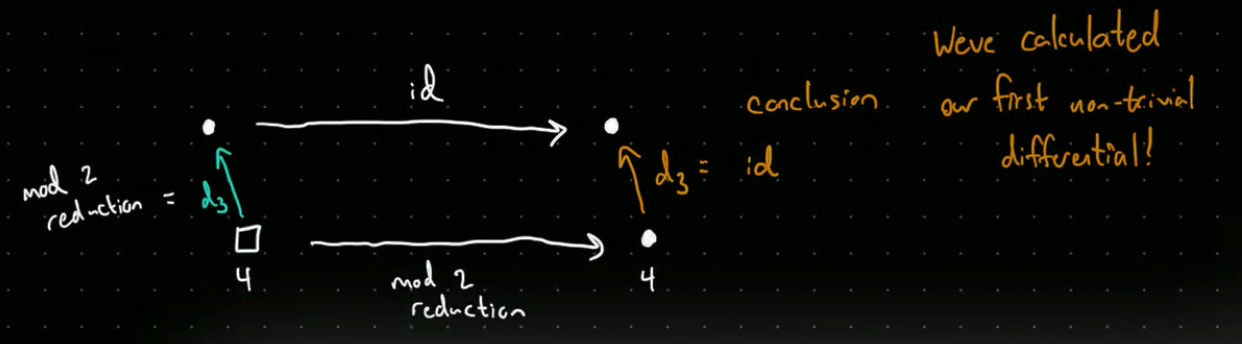
\includegraphics[width = 4in]{screenshotjune13.png}
\end{center}

\begin{proposition}{}{}
    We have a tower of nontrivial differentials as shown in the image above. 
\end{proposition}
\begin{proof}
    Either do direct calculation or use the $\pi_\ast \mS$-module structure to figure it out. 
\end{proof}

\begin{sseqdata}[name = ewedgev0calculation,Adams grading]
    \tenamwednesday(0,0)
    \tenamwednesday(-8,0)
    \tenamwednesday(8,0)
    \class(-1,7)
    \class(0,8)
    \class(1,9)
    \d3(0,4)
    \d3(1,5)
    \d3(2,6)
    \foreach \m in {0,...,3}{
        \d3 ({4+\m},\m)
        \d3 ({-4+\m},\m)
        \d3 ({8+\m},\m)
    }
\end{sseqdata}
\begin{center}
    \printpage[name = ewedgev0calculation,x range = {-5}{5}, y range = {0}{6},page = 3,grid = chess]

    \printpage[name = ewedgev0calculation,x range = {-5}{5}, y range = {0}{6},page = 4,grid = chess]
\end{center}
We still don't know a lot about the pink diagonal which starts at $(-2,0)$. 

We've exhausted the data of $E\to E\wedge V(0)$. 
\newpage
\begin{question}{}{}
    How can we proceed?
\end{question}
\begin{proof}[Options]$~$
    \begin{enumerate}
        \item We can use knowledge of the final answer (which we can find from the long exact sequence in $\pi_\ast(0)$ associated to the cofiber sequence $E\xr{2}E\to E\wedge V(0).$) This is a good bet!
        \item We did all of this work using $E\to E\wedge V(0)$ to get a lot of information. Why don't we also try using $E\wedge V(0)\to \Sigma E$? This is because of extending the cofiber sequence!\footnote{The Puppe sequence is a sequence of spaces that you arrive at from taking consecutive cofibers. It's slick!} Note that $\pi_t \Sigma E = \pi_{t\pm 1}E$. This is a good fact to have!
    \end{enumerate}
\end{proof}

\begin{remark}{}{}
    Suppose there exists a spectral sequence with $E_3$ page like 
    \begin{sseqdata}[name = afterhoursw1d4sseq1, Adams grading]
        \foreach \i in {0,...,6}{
            \class[fill= white](2+\i,\i)
            \class[fill = white](-2+\i,\i)
        }
        \d["?"]3(2,0)
        \d["?"]3(3,1)
    \end{sseqdata}
    \begin{center}
        \printpage[name = afterhoursw1d4sseq1,page = 3,grid = chess]
    \end{center}
    If we know that $\pi_2(E) =0$, then we can deduce that this $d_3$ differential must exist! Because if it didn't exist, then we wouldn't get that $\pi_2 = 0$. 
\end{remark}

\newpage
\begin{question}{Why is $\pi_\ast \mS$ a ring?}{}
    \textbf{Concrete answer:} How do we multiply? Suppose $\alpha\in \pi_k\mS$ and $\beta\in \pi_\ell \mS$. We can make a new element $\alpha\beta \in \pi_{k+\ell}\mS$. 

    We can represent $$\alpha = [S^{k+i}\xr{a}S^i],\quad \beta = [S^{\ell+j}\xr{b}S^{j}].$$ We can define $$\alpha\beta:=\bracks{S^{k+\ell + i+ j}\cong S^{k+i}\wedge S^{\ell + j}\xr{a\wedge b}S^i\wedge S^j\cong S^{i+j}}\in \pi_{k+\ell}\mS.$$ Furthermore, $\alpha\beta = (-1)^{\abs{\alpha}+\abs{\beta}}\beta\alpha$. This is called ``graded commutative.''

    \bigskip
    \textbf{Formal Answer:} $\mS$ is a \defindex{ring spectrum}. A ring spectrum $R$ is a spectrum with some extra data. This extra data is 
    \begin{itemize}
        \item the unit map: $\mS\xr{\eta} R$ 
        \item the multiplication map: $R\wedge R\xr{\mu}R$
    \end{itemize}
    such that several diagrams commute. 

    \medskip
    \begin{claim}{}{}
        If $R$ is a ring spectrum, then $\pi_\ast(R)$ is a ring. 
    \end{claim}
    \begin{proof}
        $\pi_k R$ = homotopy classes of maps of spectra from $\mS^k:=\Sigma^\infty S^k$. Now, if we have $\alpha = [S^k\xr[a]R]\in \pi_k R$, $\beta = [S^\ell\xr{b}R]\in \pi_\ell R$, then we can define $$\alpha\beta = \bracks{S^{k+\ell}\cong S^k\wedge S^\ell\xr{a\wedge b}R\wedge R\xr{\mu}R}\in \pi_{k+\ell}R. $$
    \end{proof}
\end{question}

\begin{question}{What is $\eta$ from all the spectral sequences we've been looking at?}{}
    $\eta$ is an element $\eta\in \pi_1\mS$. First, note that $S^3\cong \text{ unit sphere }\subset \mC^2$. Then we have a map \begin{center}
      \begin{tikzcd}[ampersand replacement = \&]
        S^3\ar[r]\& \mCP^1\cong S^2 \\ [-20pt]
        (z,w)\ar[r,mapsto] \& {[z:w]}
      \end{tikzcd}
    \end{center}
\end{question}

